\documentclass[hidelinks,11pt,dvipsnames]{article}
% xcolor commonly causes option clashes, this fixes that
\PassOptionsToPackage{dvipsnames,table}{xcolor}
\usepackage[tmargin=1in, bmargin=1in, lmargin=0.8in, rmargin=1in]{geometry}

%%%%%%%%%%%%%%%%%%%%%%%%%%%%%%%%%%%%%%%%%%%%%%%%%%%%%%%%%%%%%%%%%%%%
%%% For inkscape-figures
%%% Assumes the following directory structure:
%%% master.tex
%%% figures/
%%%     figure1.pdf_tex
%%%     figure1.svg
%%%     figure1.pdf
%%%%%%%%%%%%%%%%%%%%%%%%%%%%%%%%%%%%%%%%%%%%%%%%%%%%%%%%%%%%%%%%%%%%
%\usepackage{import}
\usepackage{pdfpages}
\usepackage{transparent}

\newcommand{\incfig}[2][1]{%
    \def\svgwidth{#1\columnwidth}
    \import{./figures/}{#2.pdf_tex}
}

\pdfsuppresswarningpagegroup=1

% enable synctex for inverse search, whatever synctex is
\synctex=1
\usepackage{float,macrosabound,homework,theorem-env}
\usepackage{microtype}


% font stuff
\usepackage{sectsty}
\allsectionsfont{\sffamily}
\linespread{1.1}

% bibtex stuff
\usepackage[backend=biber,style=alphabetic,sorting=anyt]{biblatex}
\addbibresource{main.bib}

% colored text shortcuts
\newcommand{\blue}[1]{\color{MidnightBlue}{#1}}
\newcommand{\red}[1]{\textcolor{Mahogany}{#1}}
\newcommand{\green}[1]{\textcolor{ForestGreen}{#1}}


% use mathptmx pkg while using default mathcal font
\DeclareMathAlphabet{\mathcal}{OMS}{cmsy}{m}{n}

% fixes the positioning of subscripts in $$ $$
\renewcommand{\det}{\operatorname{det}}

\usetikzlibrary{positioning, arrows.meta}
\newcommand{\here}[2]{\tikz[remember picture]{\node[inner sep=0](#2){#1}}}

%%%%%%%%%%%%%%%%%%%%%%%%%%%%%%%%%%%%%%%%%%%%%%%%%%%%%%%%%%%%%%%%%%%%%
%%% Entry Counter
%%%%%%%%%%%%%%%%%%%%%%%%%%%%%%%%%%%%%%%%%%%%%%%%%%%%%%%%%%%%%%%%%%%%%
\newcounter{entry-counter}
\newcommand{\entry}[1]
{
	\addtocounter{entry-counter}{1}
    \tchap{Entry \arabic{entry-counter}}
	%\addcontentsline{toc}{section}{Entry \arabic{entry-counter}: #1}
	\vspace{-1.5em}
    \begin{center}
		\small \emph{Written: #1}
    \end{center}
}

\usepackage{titling}
\renewcommand\maketitlehooka{\null\mbox{}\vfill}
\renewcommand\maketitlehookd{\vfill\null}


\usepackage{capt-of}
\usepackage{tikz}
\usetikzlibrary{positioning,calc,intersections,through,backgrounds, shapes.geometric, decorations.markings,arrows}

\def\sset{\subseteq}
\def\iso{\cong}
\def\gend#1{\langle #1\rangle}

\newcommand{\rightoverleftarrow}{%
  \mathrel{\vcenter{\mathsurround0pt
    \ialign{##\crcr
      \noalign{\nointerlineskip}$\longrightarrow$\crcr
      \noalign{\nointerlineskip}$\longleftarrow$\crcr
    }%
  }}%
}

\newcommand\makesphere{} % just for safety
\def\makesphere(#1)(#2)[#3][#4]{%
  % Synopsis
  % \makesphere[draw options](center)(initial angle:final angle:radius)
  \shade[ball color = #3, opacity = #4] #1 circle (#2);
  \draw #1 circle (#2);
  \draw ($#1 - (#2, 0)$) arc (180:360:#2 and 3*#2/10);
  \draw[dashed] ($#1 + (#2, 0)$) arc (0:180:#2 and 3*#2/10);
}
% same thing as makesphere but places white background behind
\newcommand\altmakesphere{} % just for safety
\def\altmakesphere(#1)(#2)(#3)[#4][#5]{%
  % Synopsis
  % \make sphere[draw options](center)(initial angle:final angle:radius)
  \draw [fill=white!30] #1 circle (#2);
  \shade[ball color = #4, opacity = #5] #1 circle (#2);
  \draw #1 circle (#2);
  \draw ($#1 - (#2, 0)$) arc (180:360:#2 and 3*#2/10);
  \draw[dashed] ($#1 + (#2, 0)$) arc (0:180:#2 and 3*#2/10);
  \node at #1 {#3};
}

\begin{document}
% set section number to 1
% fixes theorem numbering without need to have a section title
\setcounter{section}{1}

\pagestyle{empty}
	\LARGE
\begin{center}
	Foundations of Data Science and Machine Learning \\
	\Large
	Isaac Martin \\
    Last compiled \today
\end{center}
\normalsize
\vspace{-4mm}
\hru

\begin{homework}[e]
  \prob Let $X$ be a random variable with probability density 1/4 for $0 \leq X \leq 4$ and zero elsewhere.
  \begin{enumerate}[(a)]
    \item Use Markov's inequality to bound the probability that $X \geq 3$.
    \item Make use of $\Prob*(|X| \geq a) = \Prob(X^2 \geq a^2)$ to get a tighter bound.
    \item What is the bound obtained using $\Prob(|X| \geq a) = \Prob(X^r \geq a^r)$ where $r$ is a positive even integer?
  \end{enumerate}
  \begin{prf}
    \begin{enumerate}[(a)]$ $
      \item Since $X$ has a probability density function $f(x) = \frac{1}{4}\id_{[0,4]}$, $X$ is a uniformly distributed random variable and has expectation
        \begin{align*}
          \bE[X] = \int_0^4 xf(x) dx = \frac{1}{4}\left(\frac{x^2}{x}\right)^{x = 4}_{x = 0} = 2.
        \end{align*}
        Hence, by Markov's inequality, we have
        \begin{align*}
          \bP[X \geq 3] \leq \frac{\bE[X]}{3} = \frac{2}{3}.
        \end{align*}
      \item We may use the fact that $\bP[X\geq a] = \bP[X^r \geq a^r]$ to get a tighter bound on $\bP[X\geq 3]$. The moment-generating function for $X$ is $m(x) = \frac{e^{4t}-1}{4t}$, so
        \begin{align*}
          \bE[X^2] = \lim_{t\to 0} \frac{d}{dt} m(x) = \lim_{t\to 0} \frac{e^{4t}(8t^2 - 4t + 1)-1}{2t^3} = 16/3,
        \end{align*}
        so Markov gives us
        \begin{align*}
          \bP[X \geq 3] = \bP[X^2 \geq 9] = \frac{16/3}{9} = \frac{16}{27} < \frac{2}{3},
        \end{align*}
        a better bound.
      \item I'm not sure why I felt the need to use the moment generating function in part (b); we know the distribution function of $X$ so we can just calculate the $r$th moment:
        \begin{align*}
          \bE[X^r] = \int_0^4 \frac{1}{4}x^r dx = \frac{1}{4(r+1)}x^{r+1}\Big|^4_0 = \frac{4^r}{r+1}.
        \end{align*}
        Hence, Markov's inequality gives us the bound
        \begin{align*}
          \bP[|X| \geq a] = \bP[|X|^r \geq a^r] \leq \frac{\bE[|X|^r]}{a^r} = \frac{4^r}{(r+1)a^r}
        \end{align*}
        if we utilize the higher moments. 
    \end{enumerate}
  \end{prf}

  \prob A \emph{Rademacher} random variable $X$ has the probability mass function $\Prob(X = -1) = 1/2$ . Suppose that $X$ and $Y$ are independent Rademacher random variables, and form the random variable $Z = XY$. Show that the random variables $X,Y,Z$ are pairwise independent but no mutually independent.
  \begin{prf}
    We first note that $X$ and $Y$ are independent by definition and that, because $X$ and $Y$ are both Rademacher random variables, it suffices to show that $X$ and $Z$ are independent by symmetry. 
    Recall that $X$ and $Z$ are independent if the $\sigma$-algebras they generate are independent. Equivalently, they are independent if $\bP(X\leq x\textbuff{1em}{and} Z \leq z) = \bP(X\leq x)\cdot \bP(Z\leq z)$. We have that
    \begin{align*}
      \bP(X\leq x) =
      \begin{cases}
        0 & x < -1 \\
        1/2 & -1 \leq x < 1 \\
        1 & 1 \leq x
      \end{cases}
    \end{align*}
    and similarly
    \begin{align*}
      \bP(Z \leq z) = \bP(XY \leq z) =
      \begin{cases}
        0 & z < -1 \\
        1/2 & -1 \leq z < 1 \\
        1 & 1 \leq z
      \end{cases}.
    \end{align*}
    Now we calculate $\bP(X\leq x\textbuff{0.5em}{and} XY\leq z)$ by examining cases. We assume without loss of generality that $X$ and $Y$ only contain $-1$ and $1$ in their domain; if not, then we can replace $X$ and $Y$ with such functions which are almost surely equivalent. If either $x$ or $z$ is less than $-1$ then this evaluates to zero. If $-1 \leq x< 1$ then $X$ must be $-1$. If $-1 \leq z < 1$ then $XY$ also must be $-1$, meaning $Y = 1$ and $(X,Y) = (-1, 1)$. This occurs with probability $1/4$. If $z \geq 1$, then $XY = -1$ or $1$ so $Y = -1$ or $1$ and $\bP(X\leq x\textbuff{1em}{and} XY\leq z) = 1/2$. In either case, $\bP(X\leq x\textbuff{1em}{and} XY\leq z) = \bP(X \leq x)\cdot \bP(XY \leq z)$.

    For the final two cases we get probabilities of $1/2$ and 1, which also agree with the necessary product. This means $X$ and $Z$ are indeed independent, and hence so are $Y$ and $Z$.

    \bigskip

    However, the product $XYZ$ is $1$ with probability 1. This means that
    \begin{align*}
      \bE[XYZ] = 1 \neq 0 = \bE[X]\cdot \bE[Y]\cdot \bE[Z].
    \end{align*}
    Hence $XYZ$ are not mutually independent.
  \end{prf}
  \prob Consider drawing a random point $\bfx$ on the unit sphere in $\bR^d$. What is the variance of $x_1$ (i.e. The first coordinate of $\bfx$)? Bonus [1pt]: See if you can give an argument without doing integrals.
  \begin{prf}
    I first thought to uniformly sample spherical coordinates $\theta_i \in [0,\pi]$ for $1\leq i\leq d-2$ and $\theta_{d-1} \in [0,2\pi)$. This is incorrect; points on $S^{d-1}$ chosen in this way will tend to bunch points up at the poles. Instead, we utilize the spherical symmetry of the Gaussian distribution as shown in class. Let $X_1,...,X_d \sim N(0,1)$ be i.i.d. and define
    \begin{align*}
      Y_i = \frac{X_i}{\|(X_1,...,X_d)\|}.
    \end{align*}
    Then $Y = (Y_1,...,Y_d)$ lies on $S^{d-1}$ by definition and is uniformly distributed on $S^{d-1}$ as shown in class. Notice that this means
    \begin{align*}
      Y_1^2 + ... + Y_d^2 = 1 \implies \bE[Y_1^2]+...+\bE[Y_d^2] = \bE[Y_1^2 + ... + Y_d^2] = 1.
    \end{align*}
    Since the coordinates $Y_1,...,Y_d$ are identically distributed, the expectations of $Y_i^2$ are all equal and hence
    \begin{align*}
      d\cdot \bE[Y_1^2] = 1 \implies \bE[Y_1^2] = \frac{1}{d}.
    \end{align*}
    Due to spherical symmetry, $\bE[Y_1] = 0$, and so we have actually calculated the variance already: $\Var(Y_1) = \bE[(Y_1 - \bE[Y_1])^2] = \bE[Y_1^2] = 1/d$.
  \end{prf}

  \prob Consider the probability distribution $\Prob(X = 0) = 1 - 1/a$ and $\Prob(X = a) = 1/a$. Plot the probability that $X$ is greater than or equal to $a$ as a function of $a$ for the bound given by Markov's inequality, as well as the bounds given by Markov's inequality applied to $X^2$ and $X^4$.
  \begin{prf}
    We assume that $a > 1$ -- otherwise, $\Prob(X = a) = 1/a$ wouldn't make sense. Since the probability that $X \in \{0,a\}$ is $1$, the expectation of $X$ is given by
    \begin{align*}
      \bE[X] = \Prob(X=0)\cdot 0 + \Prob(X = a)\cdot a = 1.
    \end{align*}
    The higher moments of $X$ are given by
    \begin{align*}
      \bE[X^r] = \Prob(X=0)\cdot 0 + \Prob(X = a)\cdot a^r = a^{r-1}.
    \end{align*}
    This means that for $r \geq 1$ Markov yields
    \begin{align*}
      \bP[X\geq a] = \bP[X^r \geq a^r] \leq \frac{\bE[X^r]}{a^r} = \frac{a^{r-1}}{a^r} = \frac{1}{a}.
    \end{align*}
    Since $\bP[X\geq a] = \bP[X > a] + \bP[X = a] = 0 + \frac{1}{a}$, Markov's inequality is actually an \emph{equality} here.

    I'm worried that I'm missing something here, because Markov seems to tell us something weaker than what we already know: $\bP[X\geq a] = \bP[X = a] = 1/a$. Here's the figure:
    \begin{center}
      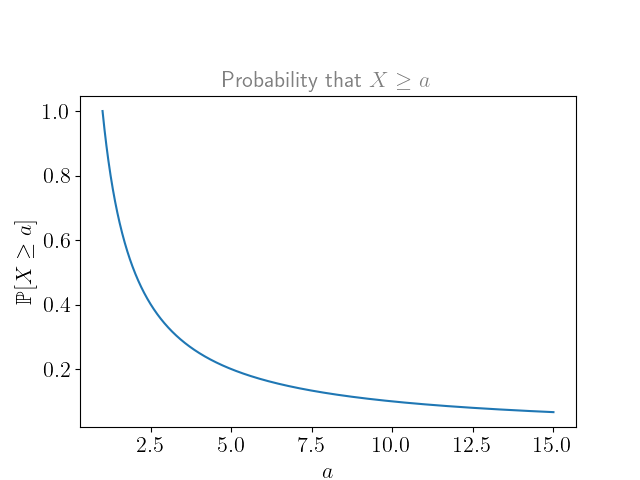
\includegraphics[width=12cm]{~/Desktop/university/code/dsml/hwk1/prob4.png}
      \captionof{figure}{Probability that $X \geq a$ plotted as a function of $a$}
      \label{fig:prob4-1}
    \end{center}
  \end{prf}

  \prob If one randomly generates points in $\bR^d$ with each coordinate a unit variance Gaussian, the points will approximately lie on the surface of a sphere of radius $\sqrt{d}$. What is the distribution when the points are projected onto the line through the origin in the direction of $(1,0,0,...,0)$? How about when they are projected onto an arbitrary line through the origin?
  \begin{prf}
    If one chooses $X_1,...,X_d \sim N(0,1)$ all i.i.d. normal random variables as in problem 3, then $X = (X_1,...,X_d)$ satisfies $X \sim N(0,I_d)$ where $I_d$ is the identity matrix. From this it follows that $OX$ is identically distributed to $X$ for any orthogonal matrix $O \in O(d)$. Thus, if $\ell$ is an arbitrary line through the origin, we may apply a rotation matrix $A$ so that $A\ell$ is the line passing through the origin and $(1,0,...,0)$ without affecting the distribution of $X$. It therefore suffices to find the distribution of $X$ projected onto the line passing through $(1,0,...,0)$ and the origin to answer both parts of this question. However, this is easy:
    $X$ projected onto this line is simply the projection of $X\mapsto X_1$, so the distribution is $N(0,1)$.
  \end{prf}

  \prob In your preferred programming language, uniformly generate 100 random points on the surface of a sphere in 3-dimensions and in 100-dimensions. Create a histogram of all distances between the pairs of points in both cases and discuss.
  \begin{soln}
    To generate points on the unit sphere we follow the same procedure as in problem 3 and 5: we sample a data point $X$ from $N(0,I_d)$ (which is equivalent to sampling the $i$th coordinate $X_i$ of $X$ from $N(0,1)$) and then normalize its components. This yields a point uniformly sampled from $S^{d-1}$, the unit sphere in $\bR^d$.

    Before we show the desired plots, we first list some observations.
    \begin{enumerate}[(1)]
      \item For any two points $x,y \in S^n$, the Euclidean distance $\|x - y\|$ falls within the interval $[0,2]$
      \item If we fix a point $x \in S^n$ and a real number $r \in [0,2]$, then the set $L_x(r)$ of all points $y \in S^n$ distance $r$ from $x$ is a copy of $S^{n-1}$ obtained by intersecting some hyperplane $H \subseteq \bR^n$ orthogonal to the line between $x$ and its antipode $-x$.
      \item There is exactly one $r \in [0,2]$ such that set $L_x(r)$ is a great circle, and it occurs for $r = \sqrt{2}$.
    \end{enumerate}
    With these claims in mind, let's see the requested plots.
    \begin{center}
      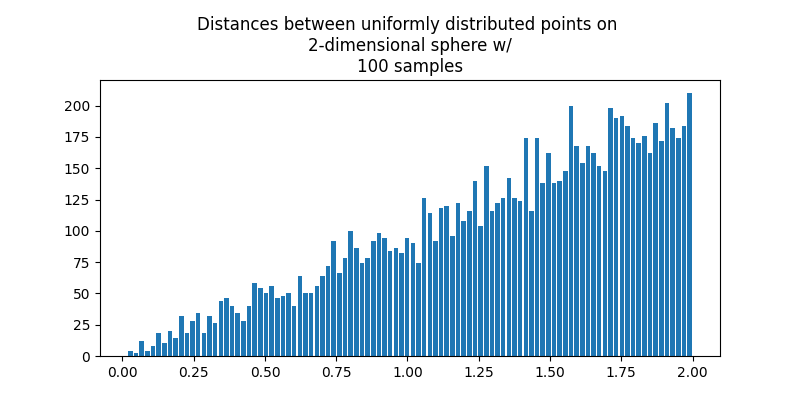
\includegraphics[width=12cm]{~/Desktop/university/code/dsml/hwk1/prob6_dim2_100samples.png}
      \captionof{figure}{Distribution of distances between points on the unit sphere in $\bR^3$}
      \label{fig:prob6-1}
    \end{center}
    \begin{center}
      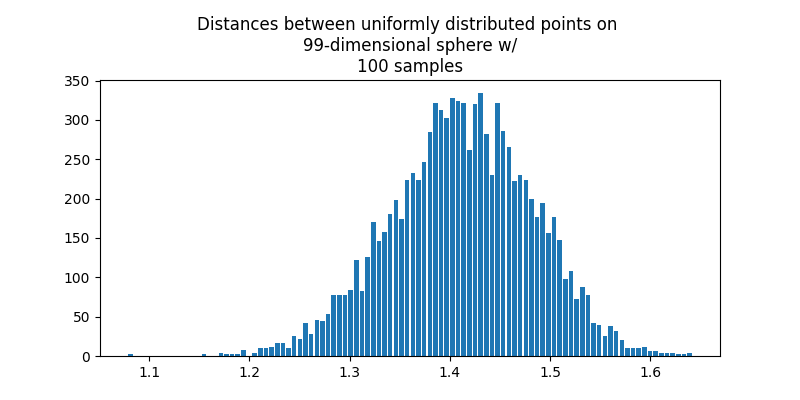
\includegraphics[width=12cm]{~/Desktop/university/code/dsml/hwk1/prob6_dim99_100samples.png}
      \captionof{figure}{Distribution of distances between points}
      \label{fig:prob6-2}
    \end{center}
    For $d = 3$ the distribution seems to be linear, while for $d = 100$ it appears to be normal. To see what's going on here, let's plot in several more dimensions with more samples.
    \begin{center}
      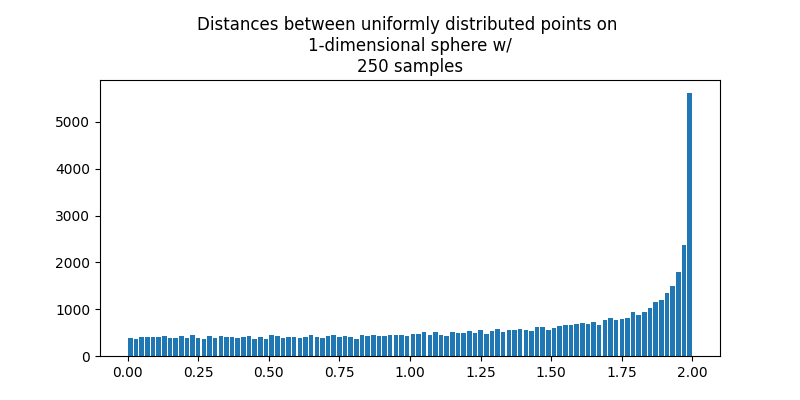
\includegraphics[width=12cm]{~/Desktop/university/code/dsml/hwk1/prob6_dim1_250samples.png}
      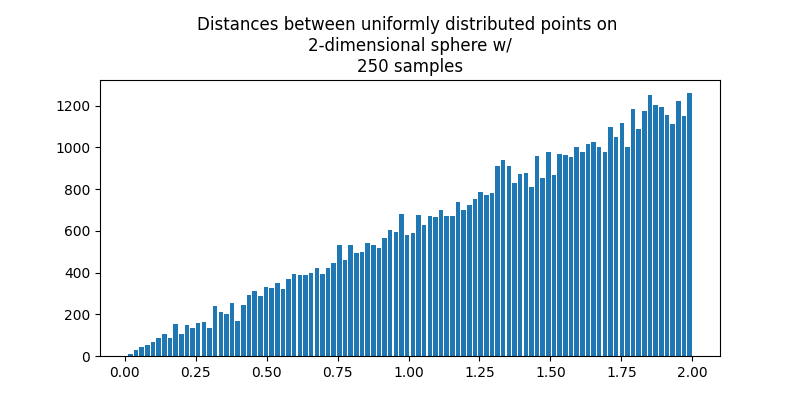
\includegraphics[width=12cm]{~/Desktop/university/code/dsml/hwk1/prob6_dim2_250samples.png}
      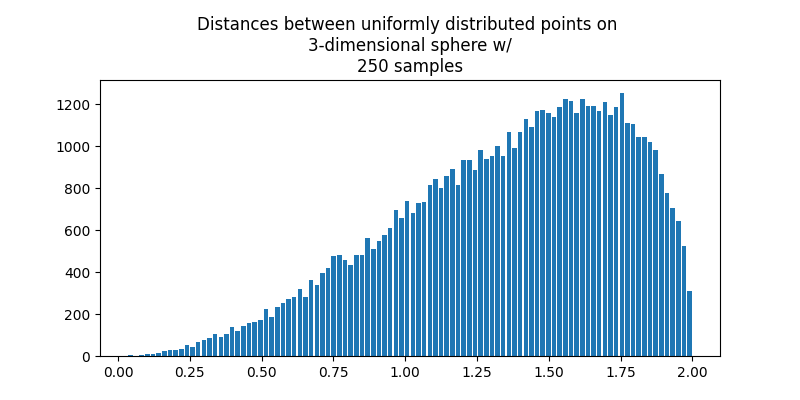
\includegraphics[width=12cm]{~/Desktop/university/code/dsml/hwk1/prob6_dim3_250samples.png}
      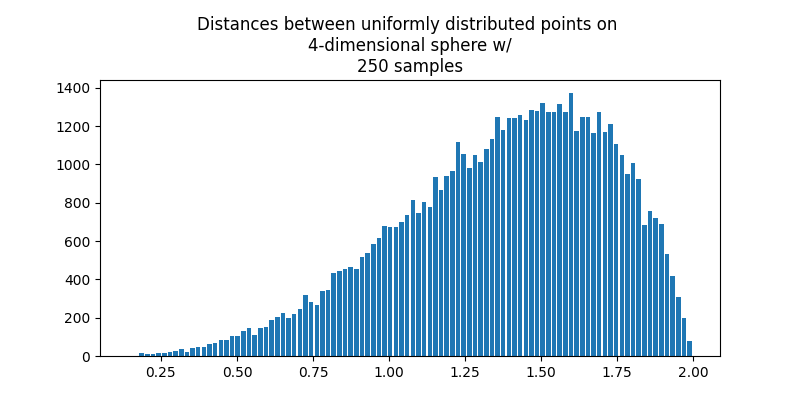
\includegraphics[width=12cm]{~/Desktop/university/code/dsml/hwk1/prob6_dim4_250samples.png}
      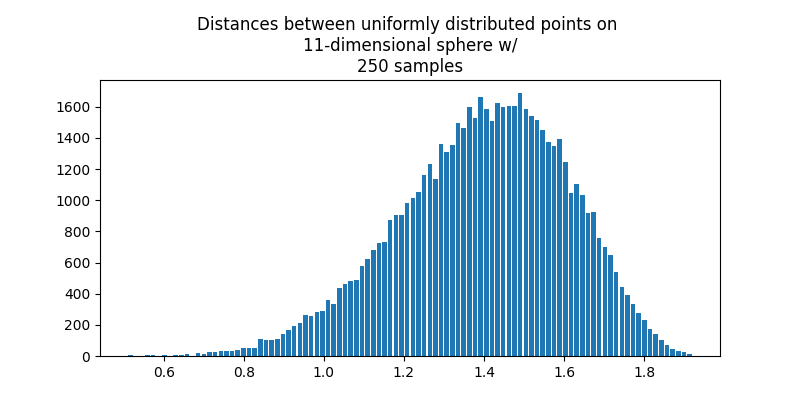
\includegraphics[width=12cm]{~/Desktop/university/code/dsml/hwk1/prob6_dim11_250samples.png}
      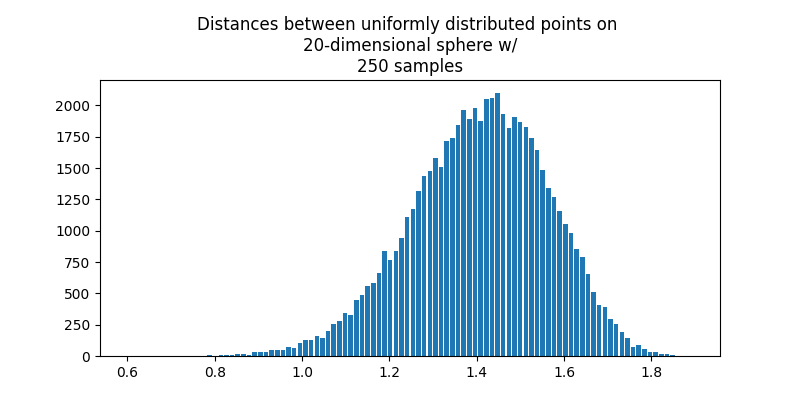
\includegraphics[width=12cm]{~/Desktop/university/code/dsml/hwk1/prob6_dim20_250samples.png}
      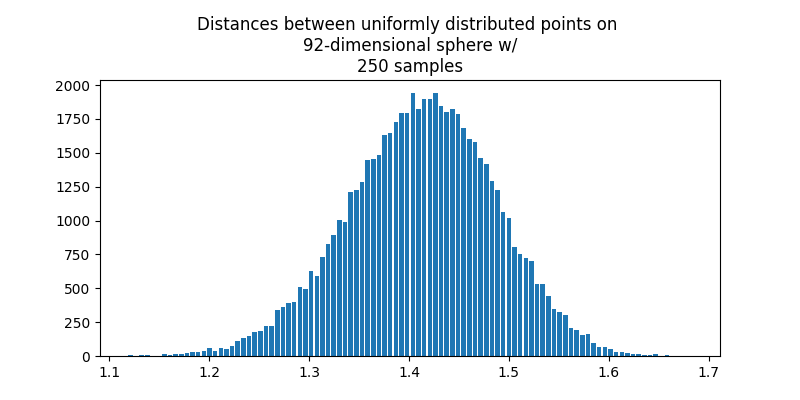
\includegraphics[width=12cm]{~/Desktop/university/code/dsml/hwk1/prob6_dim92_250samples.png}
      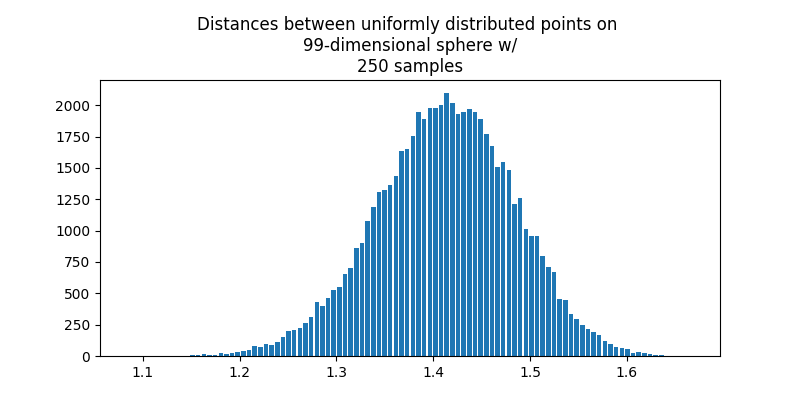
\includegraphics[width=12cm]{~/Desktop/university/code/dsml/hwk1/prob6_dim99_250samples.png}
      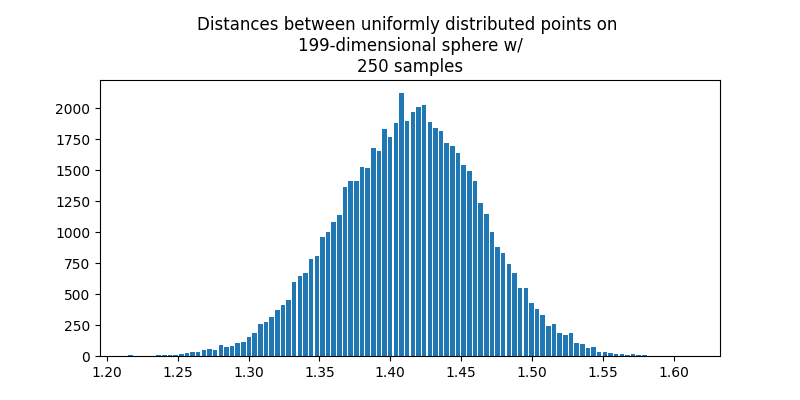
\includegraphics[width=12cm]{~/Desktop/university/code/dsml/hwk1/prob6_dim199_250samples.png}
      \captionof{figure}{Distribution of distances between points for many values of $d$}
      \label{fig:prob6-3}
    \end{center}
    It seems that as the dimension $d$ increases, the distribution of distances between uniformly sampled points on the unit sphere becomes a better approximation of a bell curve centered around $\sqrt{2}$. Of course, this isn't actually a normal distribution -- the support of our distribution is compact, $[0,2]$ -- but perhaps it's something like a truncated normal distribution in the limit. What is surprising, at least to me, is that in low dimensions we have a significant bias towards the larger distances. What's going on here?

    Consider two points $P$ and $Q$ randomly chosen on the surface of $S^{d-1}$. Since the special orthogonal group $SO_{d}$ acts isometrically on $S^{d-1}$, we can assume that $P = (1,0,...,0)$ is the north pole of $S^{d-1}$ after perhaps applying a rotation. Now consider the map $\varphi_P:S^{d-1}\to \bR$ which sends a point on the sphere to its distance from $P$: $\varphi_P(x) = \|P - x\|$. We would like to understand the level sets $L_P(a) = \varphi^{-1}_P(a)$ of this function. Actually, that's not quite right; we want to understand the measure of $L_P([a - \epsilon, a+\epsilon])$ for small $\epsilon$ as a function of $a \in [0,2]$. This should tell us the probability that two points randomly chosen on $S^{d-1}$ have a distance within $\epsilon$ of $a$.

    For small values of $d$, there are many points on $S^{d-1}$ which are far from $P$ and fewer which are close to $P$. Another way to state this is $\varphi^{-1}([a-\epsilon,a+\epsilon])$ has large measure when $a$ is large and small measure when $a$ is small. This is illustrated in Figure \ref{fig:prob6-8} and is demonstrated empirically in Figure \ref{fig:prob6-9}.
    \begin{center}
      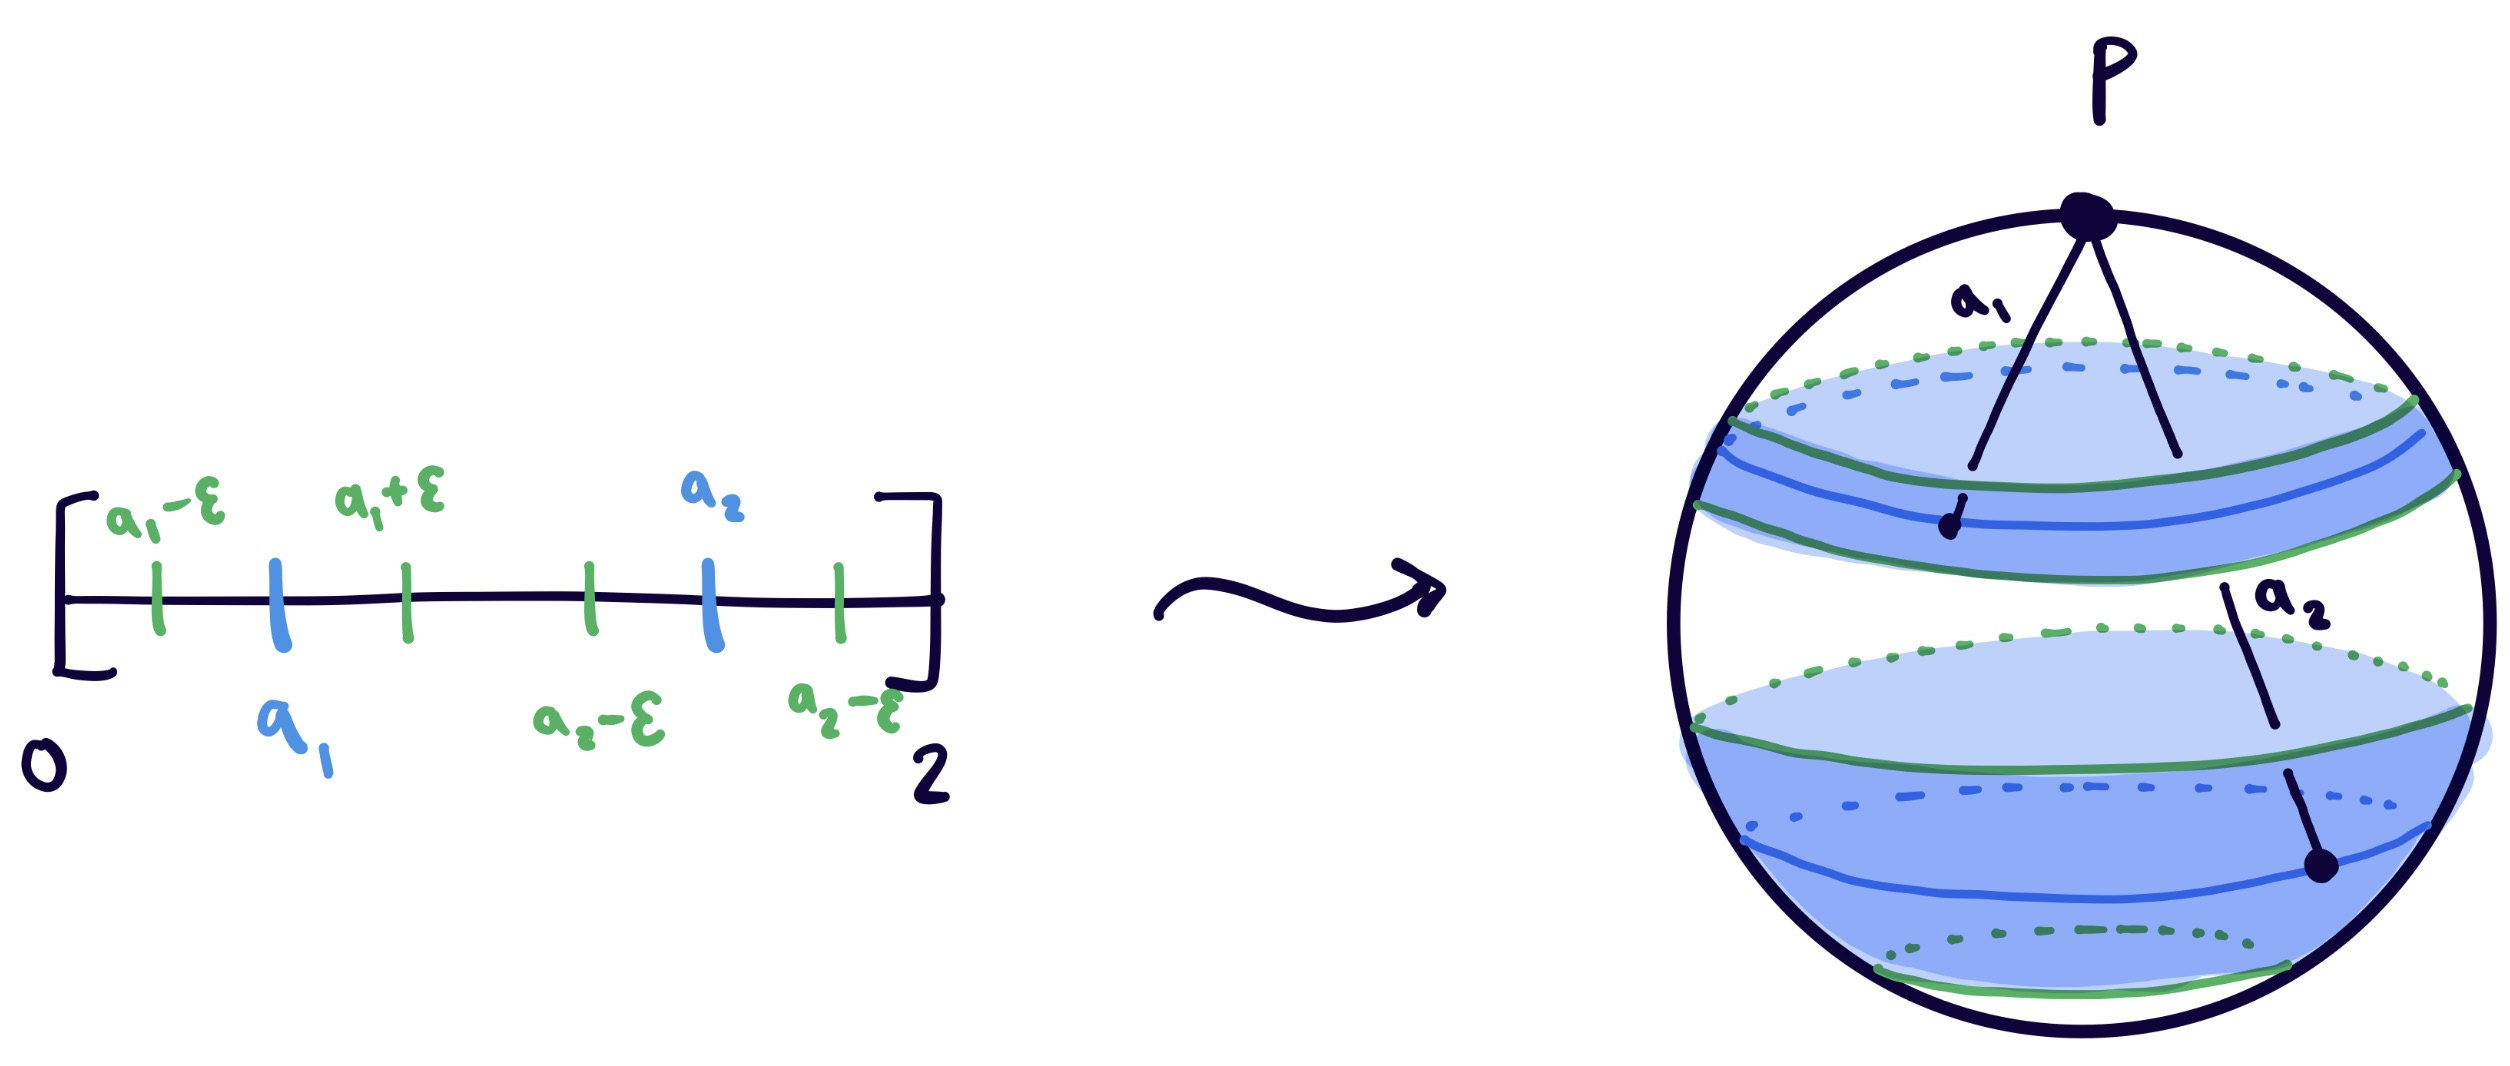
\includegraphics[width=12cm]{figures/hwk1-drawing3.png}
      \captionof{figure}{Epsilon neighborhoods around small $a$ values correspond to thin strips on the surface of $S^{d-1}$}
      \label{fig:prob6-8}
    \end{center}
    \begin{center}
      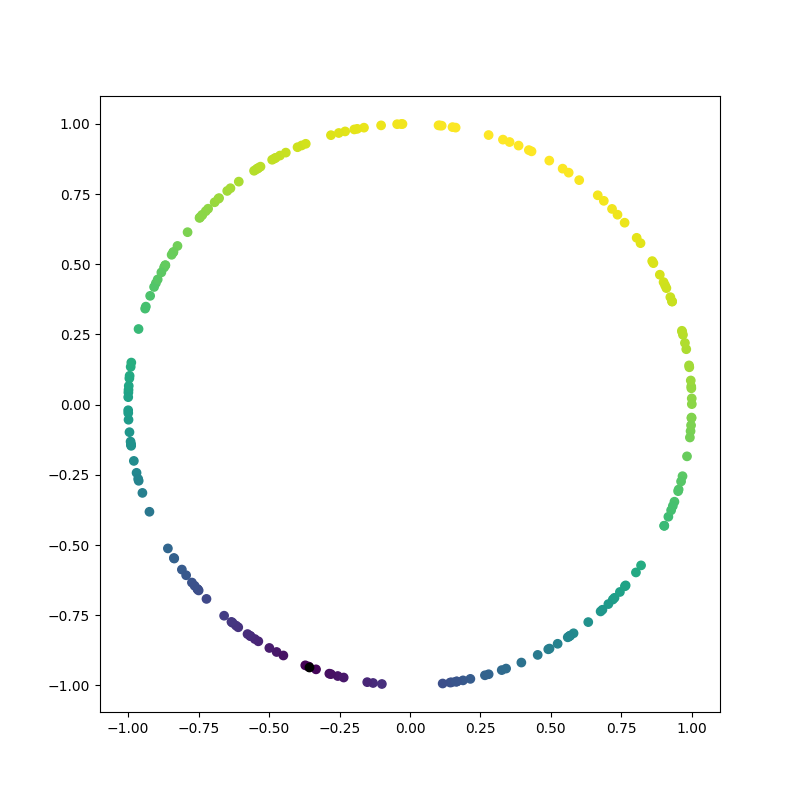
\includegraphics[width=10cm]{~/Desktop/university/code/dsml/hwk1/pointcloud_dim1.png}
      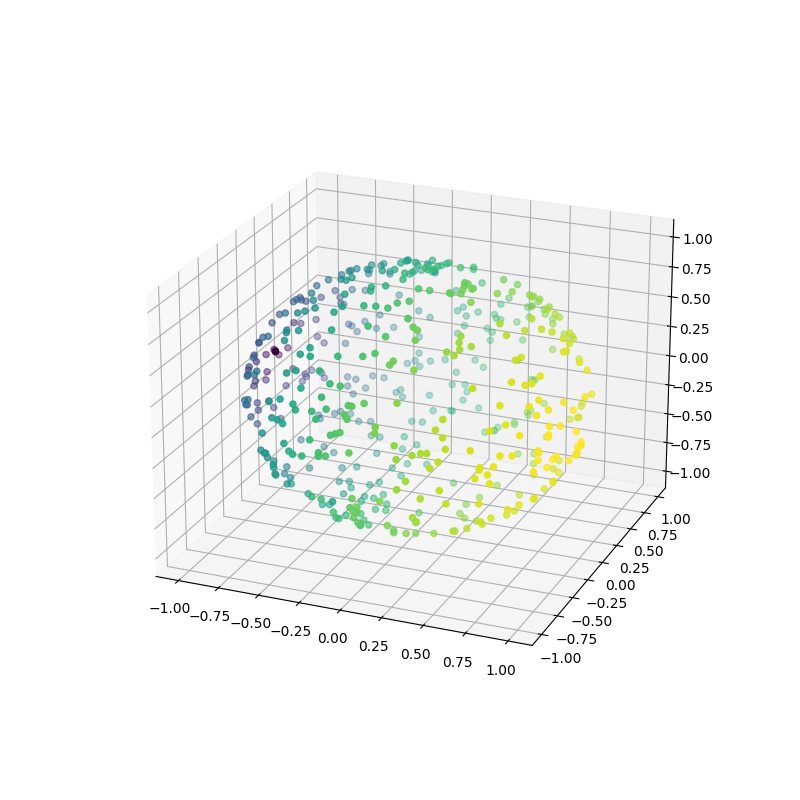
\includegraphics[width=10cm]{~/Desktop/university/code/dsml/hwk1/pointcloud_dim2.png}
      \captionof{figure}{Points uniformly distributed on $S^{d-1}$ for $d = 2,3$ colored by their distance from the black point. Violet means a point is close, yellow means a point is far.}
      \label{fig:prob6-9}
    \end{center}
    As the dimension $d$ increases however, the width of the $\epsilon$-neighborhood around $a$ and the thickness of the strip around the level set $L_P(a)$ ceases to depend as heavily on $a$. Though we have demonstrated this empirically, we have not shown it rigorously. What follows is an attempt to do that, although it got quite messy.

    As previously noted, the level set $L_P(a)\subseteq S^{d-1}$ is a $(d-2)$-dimensional sphere of some radius $R$. Hopefully the geometric intuition is clear enough (see Figure \ref{fig:prob6-4}) to claim this without proof. 
    \begin{center}
      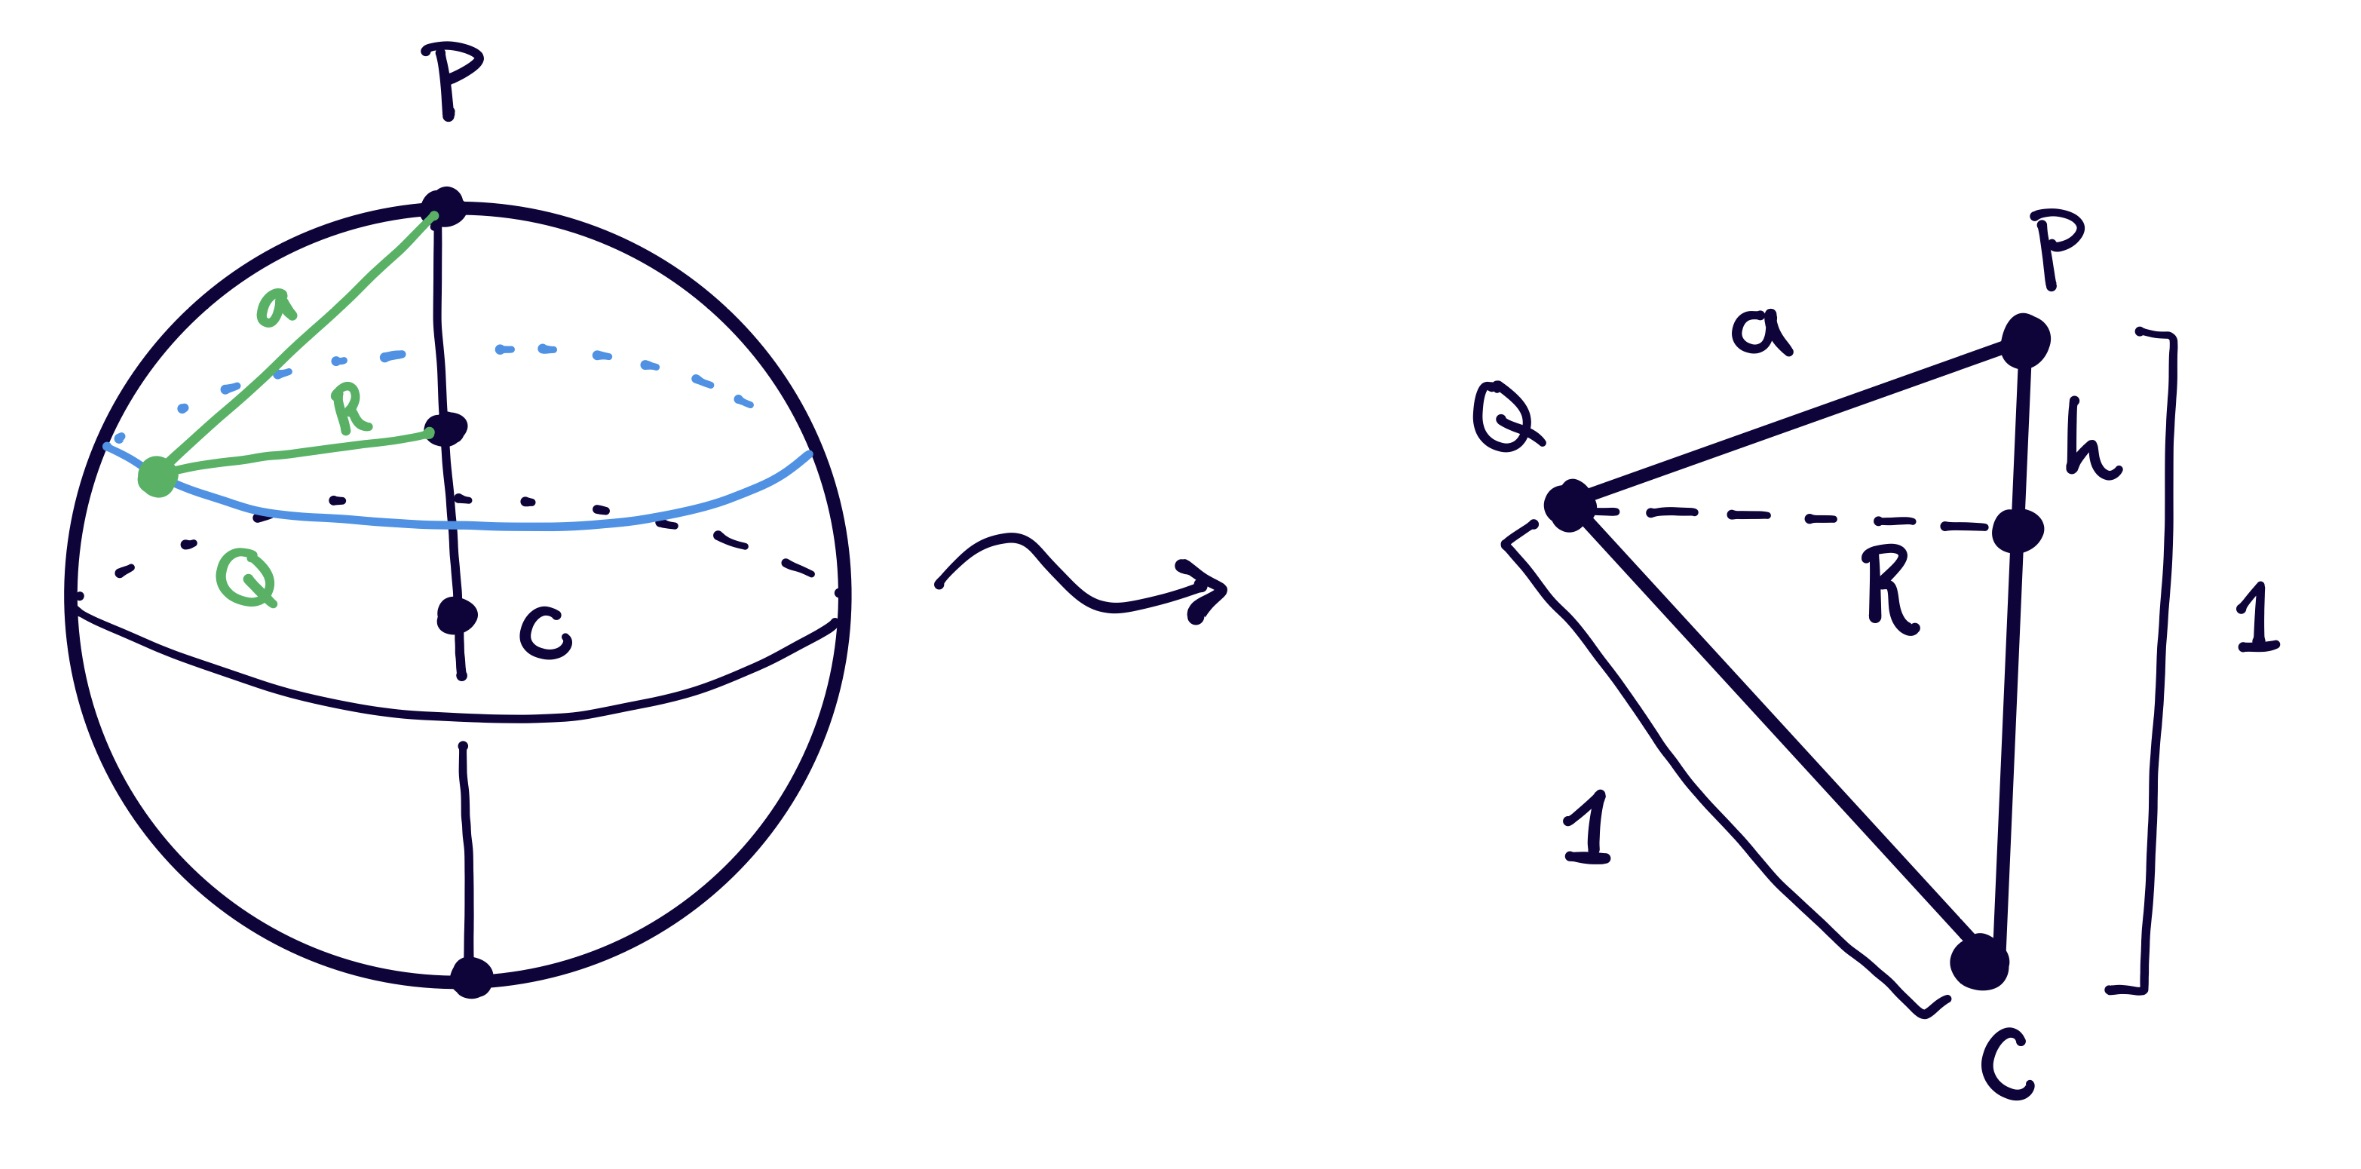
\includegraphics[width=12cm]{figures/hwk1-drawing1.png}
      \captionof{figure}{Geometric relationship between distance $a$ between $P$ and $Q$ and the spherical level set $L_P(a)$ of radius $R$, seen here in blue.}
      \label{fig:prob6-4}
    \end{center}
    The relationship between $a$ and $R$ can be derived from two applications of Pythagorean's theorem. The triangle on the right of Figure \ref{fig:prob6-4} gives us that
    \begin{align*}
      R^2 + h^2 = a^2 \textbuff{1em}{and} R^2 + (1 - h)^2 = 1^2.
    \end{align*}
    Solving for $R$ in terms of $a$ gives us
    \begin{align}\label{eqn:R-and-a}
      R^2 = a^2 - \frac{a^4}{4} \implies R = a\cdot \frac{\sqrt{4 - a^2}}{2}.
    \end{align}

    Now, we'd like to understand the measure of $L_P([a - \epsilon, a+\epsilon]) = \varphi^{-1}_P([a-\epsilon,a+\epsilon])$, which is a strip around the sphere enclosing the ``circle'' $L_P(a)$ of radius $a\cdot \sqrt{(4-a^2)/2}$. A first guess might be that
    \begin{align*}
      \mu(\varphi^{-1}_P([a-\epsilon,a+\epsilon])) \approx \mu(\varphi^{-1}_P(a)) \times 2\epsilon,
    \end{align*}
    i.e. that the surface area of the strip on the sphere is approximately the surface area of a cylinder with height $2\epsilon$ and base $\varphi^{-1}_P(a)$ (see Figure )
    \begin{center}
      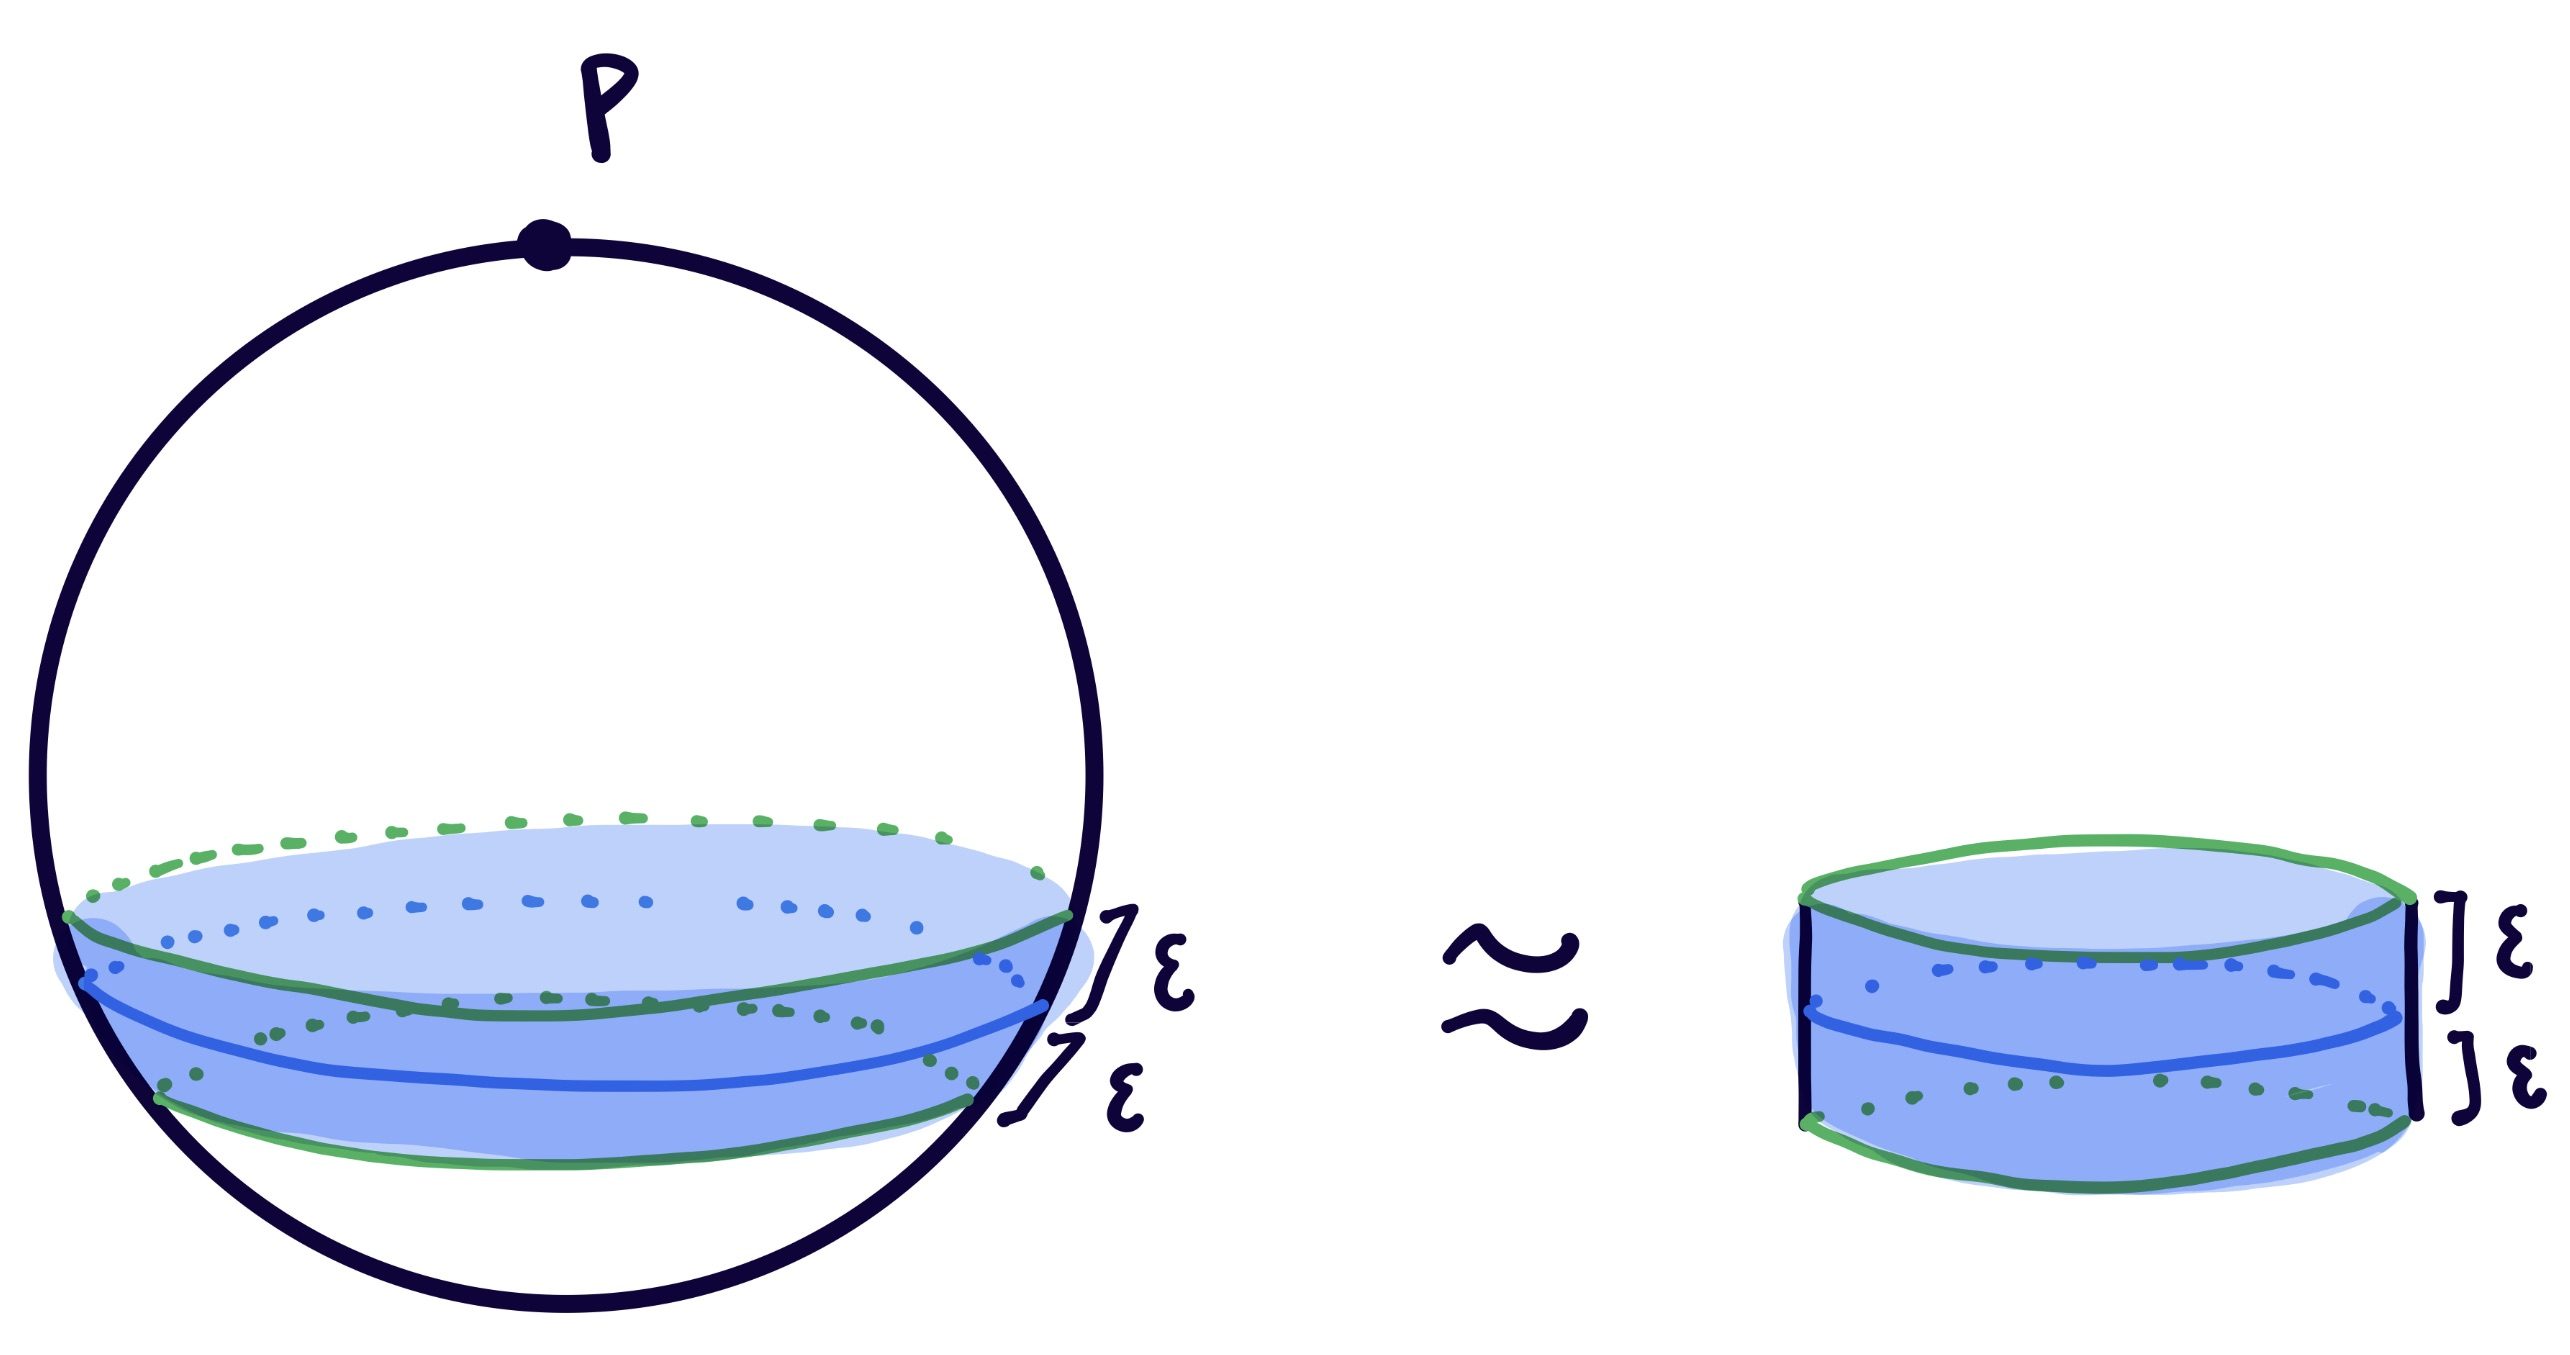
\includegraphics[width=12cm]{figures/hwk1-drawing2.png}
      \captionof{figure}{This strip of the sphere looks a lot like a cylinder}
      \label{fig:prob6-10}
    \end{center}
    The problem is that the change in height of this cylinder changes depending on the distance of the central circle $L_P(a)$ from $P$. The distance ``changes much faster'' near $P$ than it does far from $P$.

    Formalizing this a little, we see that the path $\gamma:[0,\pi]\to S^{d-1}$ defined $\gamma(\theta) = (\cos\theta,\sin\theta,0,...,0)$ has exactly one point in each level set $L_P(a)$ for $a \in [0,2]$. What's more, the path it traces is orthogonal to all of these level sets. If we denote by $a_t$ the distance between $\gamma(t)$ and $P$, then the length between $\gamma(t_2)$ and $\gamma(t_1)$ is equal to the ``height of the cylinder'' which approximates the area of the strip bounded by $L_P(a_{t_1})$ and $L_P(a_{t_2})$.

    By noticing we're simply tracing a portion of a great circle around $S^{d-1}$, we see that
    \begin{equation}\label{eqn:dist-on-great-arc}
      \frac{|t_2 - t_1|}{2\pi} = \text{ arc length between $\gamma(t_2)$ and $\gamma(t_1)$},
    \end{equation}
    and after some simplifications we get that
    \begin{align*}
      a_t^2 = 2 - 2\cos(t) \implies t = \arccos\left(1 - \frac{a_t^2}{2}\right),
    \end{align*}
    where the range of $\arccos$ is taken to be $[0,\pi]$. This is gross, so we approximate by the Taylor series of $\arccos$ to get
    \begin{align*}
      t = \frac{\pi}{2} - 1 + \frac{a_t^2}{2} - \frac{1}{6}\left(1 - \frac{a_t^2}{2}\right)^3.
    \end{align*}
    This is a good approximation when $a_t \geq 1/\sqrt{2}$, otherwise $t = |a_t|$ is a better approximation.

    We can now find the interval for $t$ which corresponds to the interval $a_t \in [a-\epsilon,a+\epsilon]$. If $a \leq 1/\sqrt{2}$, then $a_t \in [a-\epsilon,a+\epsilon]\implies t\in [1/\sqrt{2}-\epsilon, 1/\sqrt{2} + \epsilon]$. Otherwise, we have that
    \begin{align*}
      t_{\epsilon^+} &= \frac{1}{48}\left((a + \epsilon)^6 - 6(a + \epsilon)^4 + 36(a + \epsilon)^2+8(3\pi - 7)\right) \\
      t_{\epsilon^-} &= \frac{1}{48}\left((a - \epsilon)^6 - 6(a - \epsilon)^4 + 36(a - \epsilon)^2+8(3\pi - 7)\right) \\
    \end{align*}
    are the right and left endpoints of the interval. This is also disgusting, but since we're really just after the length of this interval, we'll denote it by $\delta_a = t_{\epsilon^+} - t^{\epsilon^-}$, retaining the $a$ to remind ourselves that this is really a function of $a$.
    
    \bigskip

    Putting everything together, the estimate we get for the measure of the strip on $S^{d-1}$ containing all points whose distance from $P$ is between $a - \epsilon$ and $a + \epsilon$ is
    \begin{align*}
      A = \frac{2\pi^{d/2}}{\Gamma(d/2)}R^{d-1}\cdot \delta(a)
    \end{align*}
    where $\frac{2\pi^{d/2}}{\Gamma(d/2)}R^{d-1}$ is the surface area of a $(d-2)$-dimensional sphere of radius $R$. This term is dominated by $\delta(a)$ only for small values of $d$, otherwise, its contribution is small.

    It still remains to show that in the limit $d \to \infty$ the distribution of distances between uniformly sampled points on the unit sphere in $\bR^d$ is a bell curve. If there is ample time before the submission deadline, I will try to prove this final claim and improve the previous argument. Perhaps there are some estimates that can clean up the math in places.
  \end{soln}

  \prob Suppose you wish to estimate the unknown center (i.e. mean) of a Gaussian in $d$-dimensional space with independent coordinates each with variance one. Show that $\cO(\log(d)/\epsilon^2)$ random samples from the Gaussian are sufficient to get an estimate $\hat{\mu}$ of the true center $\mu \in \bR^d$, such that with probability at least $99\%$ it holds
  \begin{align*}
    \|\mu - \hat\mu\|_\infty \leq \epsilon?
  \end{align*}
  How many samples are sufficient to ensure that with probability at least 99\% it holds
  \begin{align*}
    \|\mu - \hat\mu\|_2 \leq \epsilon?
  \end{align*}
  \begin{prf}
    This problem was by far the most fun in the set. To aid organization of the problem, we first prove some lemmas.

    \begin{lem}\label{lem:moments-normal}
      Let $X \sim N(0,1)$ be a normal random variable. Then the higher moments of $X$ are
      \begin{align*}
        \bE[X^n] =
        \begin{cases}
          0 & n \text{ is odd } \\
          \frac{1}{\sqrt{2\pi}} \Gamma\left(\frac{n+1}{2}\right) & n\text{ is even }
        \end{cases}
      \end{align*}
    \end{lem}
    \begin{proof}
      The distribution of $X$ is given by $f(x) = \frac{1}{\sqrt{2\pi}} \exp\left(-\frac{x^2}{2}\right)$, an even function. If $n$ is odd, then $x^n \cdot f(x)$ is an odd function and hence
      \begin{align*}
        \bE[X^n] &= \int_\bR x^n f ~dx \\
                 &= \int_{0}^\infty x^n f ~dx ~-~ \int_{0}^\infty x^n f ~dx = 0.
      \end{align*}
      If instead $n$ is even, then
      \begin{align*}
        \bE[X^n] &= \int_\bR x^n f ~dx
                 = \frac{2}{\sqrt{2\pi}}\int_{0}^\infty x^n e^{-x^2/2} ~dx \\
                 &= \frac{2}{\sqrt{2\pi}}\int_0^\infty u^{(n-1)/2}e^{-u}~du ~=~ \frac{1}{\sqrt{2\pi}} \cdot \Gamma\left(\frac{n+1}{2}\right).
      \end{align*}
    \end{proof}
    \begin{cor}\label{cor:normal-mtb}
      If $X_1,...,X_n$ are i.i.d. normal random variables with mean $0$ and variance $1$ then $X = \frac{1}{n}\cdot(X_1 + ... + X_n)$ satisfies the master tail bound.
    \end{cor}
    \begin{proof}
      If $s \geq 3$ is odd then we have
      \begin{align*}
        |\bE[X_i^s]| = 0 < s!
      \end{align*}
      for all $1\leq i\leq n$ by Lemma \ref{lem:moments-normal}. If instead $s = 2k \geq 3$ is even then
      \begin{align*}
        |\bE[X_i^s]| = \frac{1}{\sqrt{2\pi}} \Gamma\left(k+ \frac{1}{2}\right) = \frac{1}{\sqrt{2\pi}} \frac{(2k)!\sqrt{\pi}}{4^k\cdot k!} = \frac{s!}{\sqrt{2}\cdot 4^k \cdot (s/2)!} \leq s!,
      \end{align*}
      and hence $X$ satisfies the conditions for the master tail bound.
    \end{proof}
    Suppose now that $X_{ij} \sim N(\mu_i,1)$ is a normally distributed random variable with mean $\mu_i$ and variance $1$, that $X_i = (X_{i1},...,X_{id})$ and that $\{X_{ij}\}$ is a mutually independent collection for $1\leq j\leq d$ and $1\leq i \leq n$. That is, each $X_i$ is a point sampled from a $d$-dimensional Gaussian centered at $\mu = (\mu_1,...,\mu_d)$. Define also a random variable $\hat\mu = \frac{1}{n}\sum_{i=1}^n X_i$, the mean of the $n$ points. Note that
    \begin{align*}
      \|\mu - \hat\mu\|_{\infty} = \max_{1\leq j\leq d} |\mu_j - \hat\mu_j|,
    \end{align*}
    where $\hat\mu_j$ is the $j$th component of $\hat\mu$. 

    Choose $\epsilon > 0$. We first make the observation
    \begin{align*}
      \bP\big[\|\mu - \hat\mu\|_\infty < \epsilon\big] \geq \frac{99}{100} \iff \bP\big[\|\mu - \hat\mu\|_\infty \geq \epsilon\big] \leq \frac{1}{100}
    \end{align*}
    and
    \begin{align*}
      \bP\big[\|\mu - \hat\mu\|_\infty \geq \epsilon\big] 
      &= \bP\big[\max_{1\leq j \leq d}|\mu_j - \hat\mu_j| \geq \epsilon\big] \\
      &= \bP\Big[(|\mu_1 - \hat\mu_1| \geq \epsilon) ~\text{ OR } ~(|\mu_2 - \hat\mu_2| \geq \epsilon)~\text{ OR } ~ ... ~\text{OR}~ (|\mu_d - \hat\mu_d|\geq \epsilon)\Big]\\
      &\leq \sum_{j = 1}^d \bP\big[|\mu_j - \hat\mu_j| \geq \epsilon\big].
    \end{align*}
    We're going to apply the master tail bound to the expression above. First, we argue that we might as well assume $\mu_j = 0$ for all $1\leq j\leq d$. Define $Y_{ij} = X_{ij} - \mu_j$; then $Y_{ij} \sim N(0,1)$. If we further set
    \begin{align*}
      Z_j = \frac{1}{n}(Y_{1j} + Y_{2j}+...+Y_{nj})
    \end{align*}
    then
    \begin{align*}
      |\mu_j -\hat\mu_j| = \left|\sum_{i=1}^n(\mu_j - X_{ij})\right| = \left|-\sum_{i=1}^n Y_{ij}\right| = |Z_j|
    \end{align*}
    for all $j\in \{1..d\}$. This means that
    \begin{align*}
      \bP\big[|\mu_j-\hat\mu_j| \geq \epsilon\big] = \bP\big[|Z_j| \geq \epsilon\big]
    \end{align*}
    for all $j$. Even better, the $Z_j$ are i.i.d. since each is the mean of the $Y_{ij}$ for varying $i$, and hence
    \begin{align*} 
      \bP\big[|\mu_j-\hat\mu_j| \geq \epsilon\big] = \bP\big[|Z_j| \geq \epsilon\big] = \bP\big[|Z_{k}| \geq \epsilon\big] = \bP\big[|\mu_{k}-\hat\mu_{k}| \geq \epsilon\big]
    \end{align*}
    for all pairs $j,k \in \{1..d\}$. This implies
    \begin{align*}
      \sum_{j = 1}^d \bP\big[|\mu_j - \hat\mu_j| \geq \epsilon\big] = d\cdot \bP\big[|Z|\geq \epsilon],
    \end{align*}
    where we've chosen $Z = Z_1$ arbitrarily -- we could have defined $Z = Z_j$ for any $1\leq j\leq d$. By the Corollary, $Z = \frac{1}{n}(Y_{11} + ... + Y_{n1})$ satisfies the hypotheses of the master tail bound, so as long as we choose $\epsilon$ small enough such that $0 \leq \epsilon \leq \sqrt{2}n$ we get
    \begin{align*}
      d\cdot \bP\big[|Z|\geq \epsilon\big] = d\cdot \bP\big[|n\cdot Z|\geq n\cdot \epsilon\big] \leq d \cdot 3e^{-\frac{n^2\epsilon^2}{12n}} = 3d\cdot e^{-\frac{n\epsilon^2}{12}}.
    \end{align*}
    Notice that we've multiplied $Z$ by $n$ since $n\cdot Z = Y_{11} + ... + Y_{Y_{n1}}$, which better fits the form of the master tail bound. After completing a bit of algebra, we see that
    \begin{align*}
      3d\cdot e^{-\frac{n\epsilon^2}{12}} \leq \frac{1}{100} \textbuff{1em}{if and only if} n \geq \frac{12(\log(d) + \log(300))}{\epsilon^2}.
    \end{align*}
    Putting all this together, we conclude that for a number of samples $n$ on the order of $\cO(\log(d)/\epsilon^2)$ we have that
    \begin{align*}
      \bP\big[\|\mu - \hat\mu\|_\infty \geq \epsilon\big]  \leq \sum_{j = 1}^d \bP\big[|\mu_j - \hat\mu_j| \geq \epsilon\big] \leq 3d\cdot e^{-n\epsilon^2/12} \leq \frac{1}{100}.
    \end{align*}

    \bigskip

    Now let's consider the case of the $l^2$ norm. As we did in the last portion of the problem, we can translate our mean $\mu$ to the origin without affecting the relevant underlying probabilities; hence it suffices to assume $\mu = 0$. Suppose first that $d = 1$, in which case $\hat\mu = \sum_{i=1}^n \frac{X_i}{n}$. Squaring this yields
    \begin{align*}
      \hat\mu^2 = \frac{1}{n^2}\sum_{\substack{1\leq i\leq n\\1\leq j\leq n}} X_iX_j = \frac{1}{n^2}\sum_{i=1}^n X_i^2 ~+~ \frac{1}{n^2}\sum_{i\neq j} 2X_iX_j,
    \end{align*}
    but because the $X_i$ are independent,
    \begin{align*}
      \bE[\hat\mu^2] 
      &= \frac{1}{n^2}\bE\left[\sum_{i=1}^n X_i^2\right] ~+~ \frac{1}{n^2}\bE\left[\sum_{i\neq j} 2X_iX_j\right] \\
      &= \frac{1}{n^2}~\sum_{i=1}^n \bE[X_i^2] ~+~ \frac{1}{n^2}\sum_{i\neq j} 2\bE[X_i]\bE[X_j] = \frac{1}{n^2}~ \sum_{i=1}^n 1 = \frac{1}{n}
    \end{align*}
    since $\bE[X_i] = 0$. For arbitrary $d$, we have that
    \begin{align*}
      \bE[\hat\mu^2] =\bE[\hat\mu \cdot \hat\mu] = \bE\left[\hat\mu_1^2 + ... + \hat\mu_d^2\right] = d \cdot \bE\left[\hat\mu_1^2\right] = \frac{d}{n}
    \end{align*}
    because we can perform an identical calculation for all $\hat\mu_i$. Applying Markov's inequality yields
    \begin{align*}
      \bP[\|\hat\mu\|_2 \geq \epsilon] = \bP[\hat\mu^2 \geq \epsilon^2] \leq \frac{\bE[\hat\mu^2]}{\epsilon^2} = \frac{d}{n\epsilon^2},
    \end{align*}
    so if $\bP[\|\hat\mu\|_2 \geq \epsilon]$ is to be less than $1/100$ we must have that $n \geq \frac{100d}{\epsilon^2}$. This means we must take $\bO(100d/\epsilon^2)$ random samples to ensure with 99\% probability that $\hat\mu$ is within $\epsilon$ of the true center, measured in the $l^2$ norm.
  \end{prf}
\end{homework}
\end{document}
